\chapter[Two-Phase Navier--Stokes Flow Standard FEMs]
{\sc Standard Finite Element Approximations for Two-Phase Navier--Stokes
Flow}\label{ch:navier_stokes}
We now present two novel finite element approximations for incompressible
two-phase Navier--Stokes flow that use a fitted approach with piecewise linear
parametric finite elements to describe the moving discrete interface, and that
employ standard velocity and pressure finite element spaces in the bulk.

The chapter is organised as follows: in \S\ref{sec:ns_model} we
state the mathematical model for the incompressible two-phase Navier--Stokes
flow; in \S\ref{sec:ns_weak} we derive a standard weak formulation
and an alternative weak formulation based on an antisymmetric rewrite on which
our finite element approximations are going to be based; in
\S\ref{sec:ns_fem_antisym} we present our antisymmetric fitted finite element
discretization, we prove the existence and uniqueness of a discrete solution
and we demonstrate that this scheme has certain stability properties;
in \S\ref{sec:ns_fem} we present our standard fitted finite element
discretization; in \S\ref{sec:ns_solution_method} we explain the various
solutions methods used to solve the algebraic system; in
\S\ref{sec:ns_velocity_interpolation} we examine the techniques used to
interpolate the velocity.

\section{Mathematical model}\label{sec:ns_model}
We now consider two-phase Navier--Stokes flow in a given domain
$\Omega\subset\R^d$, where $d=2$ or $d=3$. As already described in
\S\ref{sec:free_boundary_flows} and \S\ref{sec:stokes_model}, the domain
$\Omega$ contains two different immiscible, incompressible fluids
(liquid-liquid or liquid-gas) which for all $t\in[0,T]$ occupy time
dependent regions $\Omega_+(t)$ and
$\Omega_-(t):=\Omega\setminus\overline{\Omega}_+(t)$ and which are separated by
an interface $(\Gamma(t))_{t\in[0,T]}$, $\Gamma(t)\subset\Omega$.
Consistently with two-phase Stokes flow, we limit ourselves to interfaces
formed by closed hypersurfaces, see Figure~\ref{fig:two_phase_sketch}
for a pictorial representation in dimension $d=2$.

We treat the interface $\Gamma(t)$ with the same technique used for the
two-phase Stokes, see Chapter~\ref{ch:stokes}. Therefore we use a front tracking
approach, see \S\ref{sec:front_tracking_approach}, which parametrizes the
unknown interface $\Gamma(t)$ as $\vec x(\cdot,t):\Upsilon\to\R^d$ where
$\Upsilon\subset\R^d$ is a given reference manifold such that $\Gamma(t) = \vec
x(\Upsilon,t)$. As usual, we require that the evolving hypersurface is
sufficiently smooth and without boundary. The velocity $\V$ of $\Gamma(t)$ is
defined by the equation (\ref{eq:V}) which we report here for the sake of
completeness
\begin{equation*}
\V(\vec z, t) := \vec x_t(\vec q, t) \quad
\forall\ \vec z = \vec x(\vec q,t) \in \Gamma(t)\,,
\end{equation*}
where $\V \,.\,\vec \nu$ is the normal velocity of the evolving hypersurface
$\Gamma(t)$, and $\vec\nu(t)$ is the unit normal on $\Gamma(t)$ pointing into
$\Omega_+(t)$.

The fluid dynamics in the bulk domain $\Omega$ is governed by the two-phase
Navier--Stokes model (\ref{eq:ns_momentum_bis}--b), which describes the velocity
$\vec u$ and pressure $p$ fields of the fluid. The velocity and stress tensor,
see (\ref{eq:stress_tensor}), need to be coupled across the free surface
$\Gamma(t)$. Therefore we impose the interface conditions
(\ref{eq:interface_jump_velocity}), (\ref{eq:interface_jump_stress}) and
(\ref{eq:interface_velocity}). In order to close the system, we prescribe the
initial data $\Gamma(0) = \Gamma_0$ and the initial velocity
$\vec u(0) = \vec u_0$. Finally, we impose the Dirichlet condition $\vec u =
\vec g$ on $\partial_1 \Omega$ and the free-slip condition $\vec u \,.\,\unitn =
0$ and $\mat\sigma\,\unitn\,.\,\unitt = 0$, $\forall \unitt \in
\{\unitn\}^\perp$, on $\partial_2 \Omega$, with $\unitn$ denoting the outer
unit normal of $\partial \Omega$ and $\{\unitn\}^\perp := \{ \unitt \in \R^d :
\unitt \,.\,\unitn = 0\}$. As usual, it holds that
$\partial\Omega =\partial_1\Omega \cup \partial_2\Omega$ and $\partial_1\Omega
\cap \partial_2\Omega = \emptyset$. Therefore the total system of equations
can be rewritten as follows:
\begin{subequations}
\begin{alignat}{2}
\rho\,(\vec u_t +(\vec u \,.\, \nabla)\vec u) -2 \mu\,\nabla\,.\,\mat D(\vec u)+
\nabla\,p & = \vec f
\quad &&\mbox{in } \Omega_\pm(t)\,, \label{eq:ns_full_momentum} \\
\nabla\,.\,\vec u & = 0 \quad &&\mbox{in } \Omega_\pm(t)\,,
\label{eq:ns_full_mass} \\
\vec u & = \vec g \quad &&\mbox{on } \partial_1\Omega\,,
\label{eq:ns_full_dirichlet} \\
\vec u \,.\,\unitn = 0 \,,\quad \mat\sigma\,\unitn\,.\,\unitt & = 0
\quad\forall \unitt \in \{\unitn\}^\perp \quad && \mbox{on } \partial_2\Omega\,,
\label{eq:ns_full_freeslip}\\
[\vec u]_-^+ & = \vec 0 \quad &&\mbox{on } \Gamma(t)\,,
\label{eq:ns_full_jump_velocity} \\
[2\mu \,\mat D(\vec u)\,.\,\vec\nu - p\,\vec \nu]_-^+
& = -\gamma\,\varkappa\,\vec\nu
\quad &&\mbox{on } \Gamma(t)\,, \label{eq:ns_full_jump_stress} \\
(\V-\vec u)\,.\,\vec \nu & = 0
\quad &&\mbox{on } \Gamma(t)\,,\label{eq:ns_full_velocity}  \\
\Gamma(0) & = \Gamma_0 \,,\label{eq:ns_full_initial_interface} \\
\vec u(0) & = \vec u_0 \,.\label{eq:ns_full_initial_velocity}
\end{alignat}
\end{subequations}
As usual, let $\rho(t) = \rho_+\,\charfcn{\Omega_+(t)}+
\rho_-\,\charfcn{\Omega_-(t)}$, with $\rho_\pm \in \R_{>0}$, be the fluid
density in the two phases, let $\mu(t) = \mu_+\,\charfcn{\Omega_+(t)} +
\mu_-\,\charfcn{\Omega_-(t)}$, with $\mu_\pm \in \R_{>0}$, be the dynamic
viscosities in the two phases, let $\mat D(\vec u):=\frac12\, (\nabla\vec
u+(\nabla\vec u)^T)$ be the rate-of-deformation tensor, let
$\vec f:=\rho\,\vec f_1+\vec f_2$ be a possible forcing term, let $\gamma>0$ be
the surface tension coefficient and let $\varkappa$ be the mean curvature of
$\Gamma(t)$. See Chapter~\ref{ch:introduction} for more details.

\section{Weak formulation}\label{sec:ns_weak}
A standard weak formulation of (\ref{eq:ns_full_momentum}--i) can be obtained
by proceeding analogously to the Stokes case, see \S\ref{sec:stokes_weak}. We
define the same function spaces
\begin{align*}
\uspace b &:= \{\vec \phi\in[H^1(\Omega)]^d:
\vec \phi =\vec b\quad \mbox{on }\partial_1\Omega\,,
\quad \vec \phi\,.\,\unitn=0 \quad \mbox{on }\partial_2\Omega\}\,,\\
\pspace &:= L^2(\Omega)\,,\\
\pnormspace &:= \{\eta\in\pspace : \int_\Omega\eta\dL{d}=0 \}\,,
\end{align*}
for a given $\vec b \in [H^1(\Omega)]^d$. As usual, let $(\cdot,\cdot)$ and
$\langle \cdot, \cdot \rangle_{\Gamma(t)}$ denote the $L^2$--inner products on
$\Omega$ and $\Gamma(t)$, respectively. In addition, we let $\vol$ and
$\surfvol$ denote the Lebesgue measure in $\R^d$ and the $(d-1)$-dimensional
Hausdorff measure, respectively.

Using (\ref{eq:weak_nabs_id}) and (\ref{eq:weak_stress_jump}), we can write the
standard weak formulation of (\ref{eq:ns_full_momentum}--i) as follows. Given
$\Gamma(0) = \Gamma_0$ and $\vec u = \vec u_0$, for almost all $t\in(0,T)$ find
$\Gamma(t)$ and ${(\vec u, p, \varkappa)}$ ${\in \uspace g \times \pnormspace
\times H^1(\Gamma(t))}$ such that
\begin{subequations}
\begin{align}
& \left(\rho\,\vec u_t, \vec \xi\right) + \left(\rho\,(\vec u \,.\, \nabla) \vec
u,\vec \xi\right) + 2\left(\mu\,\mat D(\vec u), \mat D(\vec \xi)\right)
\nonumber \\
& \qquad - \left(p, \nabla\,.\,\vec \xi\right)
- \gamma\,\left\langle \varkappa\,\vec\nu, \vec\xi\right\rangle_{\Gamma(t)}
= \left(\vec f, \vec \xi\right)\quad \forall\ \vec\xi \in \uspace 0 \,,
\label{eq:ns_weaka}\\
& \left(\nabla\,.\,\vec u, \varphi\right) = 0
\quad \forall\ \varphi \in \pnormspace\,, \label{eq:ns_weakb} \\
&  \left\langle \V
- \vec u, \chi\,\vec\nu \right\rangle_{\Gamma(t)} = 0
\quad \forall\ \chi \in H^1(\Gamma(t))\,, \label{eq:ns_weakc} \\
& \left\langle \varkappa\,\vec\nu, \vec\eta \right\rangle_{\Gamma(t)}
+ \left\langle \nabs\,\vec \id, \nabs\,\vec \eta \right\rangle_{\Gamma(t)}
= 0  \quad \forall\ \vec\eta \in [H^1(\Gamma(t))]^d\,\label{eq:ns_weakd}
\end{align}
\end{subequations}
holds for almost all times $t \in (0,T]$. Again, we notice that if
$p \in \pspace$ is part of a solution to (\ref{eq:ns_full_momentum}--i), then
so is $p + c$ for an arbitrary $c\in \R$.

An alternative to the weak formulation (\ref{eq:ns_weaka}--d) can be obtained
following the paper \cite{fluidfbp}. The authors show that it is easy to derive
an energy bound not only on the continuous level but also on the discrete
level. Moreover, they are able to show existence/uniqueness results for the
discrete solution. In order to obtain this
alternative weak formulation, we want to rewrite the term $\left(\rho\,\vec u_t,
\vec \xi\right) + \left(\rho\,(\vec u \,.\, \nabla) \vec u,\vec \xi\right)$ in
(\ref{eq:ns_weaka}) in such a way that certain undesirable terms vanish when
choosing $\vec \xi = \vec u$. Due to the resulting structure of the equation,
we will refer to this form as the antisymmetric weak formulation.

First, we observe that for arbitrary functions $\vec v$,
$\vec \omega$, $\vec \xi \in [H^1(\Omega)]^d$ it holds that
\begin{align}\label{eq:tripleterm}
& [(\vec v\,.\,\nabla)\,\vec \omega]\,.\,\vec \xi
 = (\vec v\,.\,\nabla)\,(\vec \omega\,.\,\vec \xi) -
[(\vec v\,.\,\nabla)\,\vec \xi]\,.\,\vec \omega \nonumber \\
& \qquad = \tfrac{1}{2}\,(\vec v\,.\,\nabla)\,
(\vec \omega\,.\,\vec \xi) + \tfrac{1}{2}\,(\vec v\,.\,\nabla)\,
(\vec \omega\,.\,\vec \xi) -\tfrac{1}{2}[(\vec v\,.\,\nabla)\,\vec
\xi] \,.\,\vec \omega -\tfrac{1}{2}[(\vec v\,.\,\nabla)\,\vec
\xi] \,.\,\vec \omega \nonumber \\
& \qquad = \tfrac{1}{2}\,(\vec v\,.\,\nabla)\, (\vec \omega\,.\,\vec \xi) +
\tfrac{1}{2}[(\vec v\,.\,\nabla)\,\vec \omega]\,.\,\vec \xi -
\tfrac{1}{2}[(\vec v\,.\,\nabla)\,\vec \xi] \,.\,\vec \omega\,.
\end{align}

Choosing $\vec v = \vec \omega = \vec u$ in (\ref{eq:tripleterm}) and
substituting it in the convection term $\left(\rho\,(\vec u \,.\, \nabla)
\vec u,\vec \xi\right)$, we obtain
\begin{equation}\label{eq:ns_advect_tripleterm}
( \rho\,(\vec u \,.\,\nabla)\,\vec u, \vec \xi) =
\tfrac{1}{2}(\rho,(\vec u\,.\,\nabla)(\vec u\,.\,\vec \xi))
+ \tfrac{1}{2}(\rho\,(\vec u \,.\,\nabla)\,\vec u, \vec \xi)
-\tfrac{1}{2}(\rho\,(\vec u\,.\,\nabla)\,\vec \xi,\vec u)\,.
\end{equation}

Then we have for any $\vec v \in [H^1(\Omega)]^d$ and
$\phi\in W_0^{1,\frac{3}{2}}(\Omega)$ that
\begin{align}\label{eq:ibp0}
( \rho,(\vec v \,.\,\nabla)\,\phi) & = (\rho, \nabla\,.\,(\phi\,\vec v))
- (\rho\,(\nabla\,.\,\vec v), \phi) \nonumber \\ & =
- \left\langle [\rho]_-^+\,\vec v\,.\,\vec \nu,
  \phi \right\rangle_{\Gamma(t)}
- (\rho\,(\nabla\,.\,\vec v), \phi)\,.
\end{align}
Here we notice that (\ref{eq:ibp0}) is well defined. Indeed, $\phi\in
W_0^{1,\frac{3}{2}}(\Omega)$ implies that its trace is in
$L^{\frac{3}{2}}(\partial\Omega)$. Moreover, given that
$\vec v \in [H^1(\Omega)]^d$, it holds that $\vec v\,.\,\vec\nu \in
H^{\frac{1}{2}}(\partial\Omega)$, which implies, thanks to the continuous
embedding theorems \cite[Theorem~6.5 and 6.7]{DINEZZA2012}, that $\vec
v\,.\,\vec\nu \in L^4(\partial\Omega)$. But we know, using the
H\"{o}lder inequality, that the term $\left\langle [\rho]_-^+\,\vec v\,.\,
\vec \nu, \phi \right\rangle_{\Gamma(t)}$ is well defined if
$\vec v\,.\,\vec\nu$ is at least in $L^3(\partial\Omega)$, which is indeed the
case.

Moreover, if $\vec u\in [H^1(\Omega)]^d$ and $\vec \xi \in \uspace{0}$ then
$\vec u\,.\,\vec\xi \in W_0^{1,\frac{3}{2}}(\Omega)$. Indeed, $H^1(\Omega)$ is
compactly embedded in $L^6(\Omega)$, for $d=2$ or $d=3$. By the
generalized H\"{o}lder inequality we know that $(\nabla h)\,\omega\in
[L^{\frac{3}{2}}(\Omega)]^d$ if $h\in H^1(\Omega)$ and $\omega\in L^6(\Omega)$.
Therefore $\nabla\,(\vec u\,.\,\vec \xi)\in [L^{\frac{3}{2}}(\Omega)]^d$,
which implies
$\vec u\,.\,\vec \xi \in W_0^{1,\frac{3}{2}}(\Omega)$. Hence, it follows from
taking $\phi = \vec u\,.\,\vec\xi$ and $\vec v = \vec u$ in (\ref{eq:ibp0}) and
applying it to the first term on the right-hand side of
(\ref{eq:ns_advect_tripleterm}) that
\begin{align}\label{eq:fulladvect}
( \rho\,(\vec u \,.\,\nabla)\,\vec u, \vec \xi) = &
-\tfrac{1}{2}\langle [\rho]_-^+\vec u\,.\,\vec \nu, \vec u\,.\,\vec \xi
\rangle_{\Gamma(t)}
-\tfrac{1}{2}(\rho\,(\nabla\,.\,\vec u ),\vec u\,.\,\vec\xi) \nonumber \\
& \qquad +\tfrac{1}{2}(\rho\,(\vec u\,.\,\nabla)\,\vec u, \vec \xi)
-\tfrac{1}{2}(\rho\,(\vec u\,.\,\nabla)\,\vec \xi,\vec u)
\quad \forall\ \vec \xi \in \uspace 0\,,
\end{align}
and, using the incompressibility condition (\ref{eq:ns_full_mass}), we obtain
\begin{align}\label{eq:advect}
( \rho\,(\vec u \,.\,\nabla)\,\vec u, \vec \xi)
= & \tfrac{1}{2} [ (\rho\,(\vec u\,.\,\nabla)\,\vec u, \vec \xi) -
(\rho\,(\vec u\,.\,\nabla)\,\vec \xi,\vec u) \nonumber \\
& \qquad -\langle [\rho]_-^+\vec u\,.\,\vec \nu, \vec u\,.\,\vec \xi
\rangle_{\Gamma(t)}] \quad \forall\ \vec \xi \in \uspace 0\,.
\end{align}

Next, we recall the Reynolds transport theorem
\begin{equation}\label{eq:reynolds_theorem}
\ddt \int_{\Omega(t)} h\dL{d}=\int_{\Omega(t)} h_t \dL{d} +
\int_{\Omega(t)} \nabla\,.\,\left(h\,\W\right)\dL{d}\,,
\end{equation}
where $\Omega(t)$ is a moving domain with velocity $\W$ and $h:\R^d\to\R$ is a
continuously differentiable function, see \cite{Aris89}. Then we can use
(\ref{eq:reynolds_theorem}) together with (\ref{eq:ns_full_velocity}), to
rewrite the time derivative term $(\rho\,\vec u_t,\vec \xi)$ and obtain
\begin{align}\label{eq:rhot1}
\ddt(\rho \,\vec u, \vec \xi) & =
\ddt\left(\rho_+\,\int_{\Omega_+(t)} \vec u \,.\,\vec \xi \dL{d}
+ \rho_-\,\int_{\Omega_-(t)} \vec u\,.\,\vec \xi \dL{d}  \right) \nonumber \\
& =  (\rho\,\vec u_t, \vec \xi)
-\left\langle [\rho]_-^+\,\V\,.\,\vec\nu, \vec u \,.\,\vec \xi
\right\rangle_{\Gamma(t)} \nonumber \\
&= (\rho\,\vec u_t, \vec \xi)- \left\langle [\rho]_-^+\,\vec u\,.\,\vec \nu,
\vec u \,.\,\vec \xi \right\rangle_{\Gamma(t)}
\quad \forall \vec \xi \in \uspace 0\,.
\end{align}
Therefore, it follows from (\ref{eq:rhot1}) that
\begin{equation*}
(\rho\,\vec u_t, \vec \xi) =
\tfrac{1}{2} \left[
\ddt (\rho\,\vec u,\vec \xi) + (\rho\,\vec u_t, \vec \xi)
+ \left\langle [\rho]_-^+\,\vec u\,.\,\vec \nu,
\vec u \,.\,\vec \xi \right\rangle_{\Gamma(t)}
\right]
\quad \forall\ \vec \xi \in \uspace 0\,,
\end{equation*}
which on combining with (\ref{eq:advect}) yields that
\begin{align} \label{eq:rhot3}
& (\rho\,[\vec u_t + (\vec u\,.\,\nabla)\,\vec u], \vec \xi) \nonumber \\
& = \tfrac{1}{2}\bigg[ \ddt (\rho\,\vec u, \vec \xi)
+ (\rho\,\vec u_t, \vec \xi) + (\rho, [(\vec u\,.\,\nabla)\,\vec u]\,.\,\vec \xi
- [(\vec u\,.\,\nabla)\,\vec \xi]\,.\,\vec u) \bigg]
\quad \forall \vec \xi \in \uspace 0\,.
\end{align}

Hence, the antisymmetric weak formulation of (\ref{eq:ns_full_momentum}--i) is
given as follows. Given $\Gamma(0) = \Gamma_0$ and $\vec u = \vec u_0$, for
almost all $t\in(0,T)$ find $\Gamma(t)$ and ${(\vec u, p, \varkappa)}$ ${\in
\uspace g \times \pnormspace \times H^1(\Gamma(t))}$ such that
\begin{subequations}
\begin{align}
& \tfrac{1}{2}\bigg[ \ddt (\rho\,\vec u, \vec \xi) + (\rho\,\vec u_t, \vec \xi)
+ (\rho, [(\vec u\,.\,\nabla)\,\vec u]\,.\,\vec \xi
- [(\vec u\,.\,\nabla)\,\vec \xi]\,.\,\vec u)\bigg] \nonumber \\
& \qquad +2\left(\mu\,\mat D(\vec u), \mat D(\vec \xi)\right)
- \left(p, \nabla\,.\,\vec \xi\right)\nonumber \\
& \qquad - \gamma\,\left\langle \varkappa\,\vec\nu, \vec\xi
\right\rangle_{\Gamma(t)}
= \left(\vec f, \vec \xi\right)\quad \forall\ \vec\xi \in \uspace 0 \,,
\label{eq:ns_weaka_antisym}\\
& \left(\nabla\,.\,\vec u, \varphi\right) = 0
\quad \forall\ \varphi \in \pnormspace\,, \label{eq:ns_weakb_antisym} \\
&  \left\langle \V
- \vec u, \chi\,\vec\nu \right\rangle_{\Gamma(t)} = 0
\quad \forall\ \chi \in H^1(\Gamma(t))\,, \label{eq:ns_weakc_antisym} \\
& \left\langle \varkappa\,\vec\nu, \vec\eta \right\rangle_{\Gamma(t)}
+ \left\langle \nabs\,\vec \id, \nabs\,\vec \eta \right\rangle_{\Gamma(t)}
= 0  \quad \forall\ \vec\eta \in [H^1(\Gamma(t))]^d\,\label{eq:ns_weakd_antisym}
\end{align}
\end{subequations}
holds for almost all times $t \in (0,T]$.

\section{Antisymmetric finite element approximation}\label{sec:ns_fem_antisym}
In order to obtain a fully practical finite element approximation of the
antisymmetric weak formulation (\ref{eq:ns_weaka_antisym}--d) we proceed
analogously to the Stokes case, see \S\ref{sec:stokes_fem}. For the benefit of
the reader, we state again all the hypothesis and the notations used.

Here, in order to have a consistent finite element approximation, we consider
the partitioning $t_m =m\,\tau$, $m=0,\ldots, M$, of $[0,T]$ into uniform time
steps $\tau=\frac{T}{M}$, see \cite{fluidfbp}. The uniform time step size is
needed to ensure that the discrete time derivative approximation is consistent.
Moreover, let ${\cal T}^m$, $\forall m\ge 0$, be a regular partitioning of the
domain $\Omega$ into disjoint open simplices $\sigmaO^m_j$, $j = 1 ,\ldots,
J^m_\Omega$. From now on, the domain $\Omega$ which we consider is the
polyhedral domain defined by the triangulation ${\cal T}^m$. On ${\cal T}^m$ we
define the finite element spaces
\begin{equation*}
S^m_k := \{\chi \in C(\overline{\Omega}) : \chi\!\mid_{\sigmaO^m}
\in \mathcal{P}_k(\sigmaO^m) \ \forall\ \sigmaO^m \in {\cal T}^m\}\,,
\quad k \in \mathbb{N}\,,
\end{equation*}
where $\mathcal{P}_k(\sigmaO^m)$ denotes the space of polynomials of degree $k$
on $\sigmaO^m$. Moreover, $S^m_0$ is the space of piecewise constant functions
on ${\cal T}^m$ and let $\vec I^m_k$ be the standard interpolation operator
onto $[S^m_k]^d$.

Let $\uspacedisc{g}{m}\subset\uspacesimple(\vec I_k^m\vec g)$ and
$\pspace^m\subset\pspace$ be the finite element spaces we use for the
approximation of velocity and pressure, and let $\pnormspace^m:= \pspace^m \cap
\pnormspace$. The spaces $(\uspacedisc{0}{m},\pspace^m)$ satisfy the LBB
inf-sup, see (\ref{eq:LBB}). Then, for $d=2$, possible pairs
$(\uspacedisc{0}{m},\pspace^m)$ that satisfy (\ref{eq:LBB}) are P2--P0 and
P2--(P1+P0), while for $d=3$ are the P3--(P2+P0) element and
P1$^{\mbox{\footnotesize face bubble}}$--P0. See \S\ref{sec:stokes_fem} for more
details.

We consider a fitted finite element approximation for the evolution of the
interface $\Gamma(t)$. Let $\Gamma^m\subset\R^d$ be a $(d-1)$-dimensional
polyhedral surface approximating the closed surface $\Gamma(t_m)$, $m=0
,\ldots, M$. Let $\Omega^m_+$ denote the exterior of $\Gamma^m$ and let
$\Omega^m_-$ be the interior of $\Gamma^m$, where we assume that $\Gamma^m$ has
no self-intersections. Then $\Omega = \Omega_-^m \cup \Gamma^m \cup
\Omega_+^m$, and the fitted nature of
our method implies that
\begin{equation*}
\overline{\Omega^m_+} = \bigcup_{o \in \mathcal{T}^m_+} \overline{o}
\quad\text{and}\quad
\overline{\Omega^m_-} = \bigcup_{o \in \mathcal{T}^m_-} \overline{o} \,,
\end{equation*}
where $\mathcal{T}^m = \mathcal{T}^m_+ \cup \mathcal{T}^m_-$ and
$\mathcal{T}^m_+ \cap \mathcal{T}^m_- = \emptyset$. Let $\vec \nu^m$ denote the
piecewise constant unit normal to $\Gamma^m$ such that $\vec\nu^m$ points into
$\Omega^m_+$.

In order to define the parametric finite element spaces on $\Gamma^m$, we
proceed analogously to the mean curvature flow and surface diffusion problems,
see \S\ref{sec:geometric_pdes_fem}. Therefore we assume that
$\Gamma^m=\bigcup_{j=1}^{J_\Gamma} \overline{\sigma^m_j}$, where
$\{\sigma^m_j\}_{j=1}^{J_\Gamma}$ is a family of mutually disjoint open
$(d-1)$-simplices with vertices $\{\vec q^m_k\}_{k=1}^{K_\Gamma}$. Then
we define $\Vh := \{\vec\chi \in [C(\Gamma^m)]^d:\vec\chi\!\mid_{\sigma^m_j}
\in \mathcal{P}_1(\sigma^m_j), j=1,\ldots, J_\Gamma\} =: [\Wh]^d$, where $\Wh
\subset H^1(\Gamma^m)$ is the space of scalar continuous piecewise linear
functions on $\Gamma^m$, with $\{\chi^m_k\}_{k=1}^{K_\Gamma}$ denoting the
standard basis of $\Wh$. As usual, we parametrize the new surface
$\Gamma^{m+1}$ over $\Gamma^m$ using a parametrization $\vec X^{m+1} \in \Vh$,
so that $\Gamma^{m+1} = \vec X^{m+1}(\Gamma^m)$. Finally, let
$\langle\cdot,\cdot\rangle_{\Gamma^m}^h$ be the mass lumped inner product on
$\Gamma^m$, see (\ref{eq:masslump}), and let
$\langle\cdot,\cdot\rangle_{\Gamma^m}$ denote the standard $L^2$--inner product
on $\Gamma^m$.

We need to pay particular attention to the discretization of the time
derivative in (\ref{eq:ns_weaka_antisym}). Indeed, for the discrete counterpart
of $\tfrac{1}{2} \ddt (\rho\,\vec u, \vec \xi)$ we use
\begin{equation}\label{eq:antysim_time_derivative_a}
\frac{1}{2}\left(\frac{\rho^m\,\vec U^{m+1} - I^m_0\,\rho^{m-1}
\vec I^m_2\,\vec U^m}{\tau}, \vec \xi \right)\,,
\end{equation}
while for the discrete version of $\tfrac{1}{2}(\rho\,\vec u_t, \vec \xi)$
we employ
\begin{equation}\label{eq:antysim_time_derivative_b}
\frac{1}{2}\left( I^m_0\,\rho^{m-1}\, \frac{\vec U^{m+1} - \vec I^m_2\,
\vec U^m}{\tau}, \vec \xi \right)\,.
\end{equation}
We notice that in (\ref{eq:antysim_time_derivative_b}), instead of using the
actual density $\rho^m$, we use the density at the previous time step
$\rho^{m-1}$ and we interpolate it on the current bulk grid $\Omega_\pm^m$. This
is needed to prove stability over one time step. Since
$\rho^m = \rho_+\,\charfcn{\Omega^m_+} + \rho_-\,\charfcn{\Omega^m_-}\in
S^m_0$, we can rewrite the discretization of the weak time derivative
$\tfrac{1}{2}\big[ \ddt (\rho\,\vec u, \vec \xi)+(\rho\,\vec u_t, \vec\xi)\big]$
in the simpler form
\begin{equation}
\left(\frac{\tfrac{1}{2}(I^m_0\,\rho^{m-1}+\rho^m)\,\vec U^{m+1} -
I^m_0\,\rho^{m-1} \vec I^m_2\,\vec U^m}{\tau}, \vec \xi \right)\,.
\end{equation}

Then our antisymmetric finite element approximation is given as follows. Let
$\Gamma^0$, an approximation to $\Gamma(0)$, and $\vec U^0\in
\uspacedisc{g}{0}$ be given. For $m=0,\ldots, M-1$, find $(\vec U^{m+1},P^{m+1},
\vec X^{m+1}, \kappa^{m+1}) \in \uspacedisc{g}{m}\times \pnormspace^m \times
\Vh \times \Wh$ such that
\begin{subequations}
\begin{align}
& \left(\frac{\tfrac{1}{2}(I^m_0\,\rho^{m-1}+\rho^m)\,\vec U^{m+1} -
I^m_0\,\rho^{m-1} \vec I^m_2\,\vec U^m}{\tau}, \vec \xi \right)\nonumber \\
& \qquad + \frac{1}{2}\left((\rho^m\,\vec I^m_2\,\vec U^m\,.\,\nabla)\,
\vec U^{m+1}\,,\,\vec \xi \right) - \frac{1}{2} \left((\rho^m\,
\vec I^m_2 \, \vec U^m\,.\,\nabla)\,\vec \xi\,,\,\vec U^{m+1} \right)
\nonumber \\
& \qquad + 2\left(\mu^m\,\mat D(\vec U^{m+1}), \mat D(\vec \xi) \right)
- \left(P^{m+1}, \nabla\,.\,\vec \xi\right) \nonumber \\
& \qquad - \gamma\,\left\langle
\kappa^{m+1}\,\vec\nu^m,\vec\xi\right\rangle_{\Gamma^m}
= \left(\rho^m\,\vec f_1^{m+1}+\vec f_2^{m+1}, \vec \xi\right)
\quad \forall\ \vec\xi \in \uspacedisc{0}{m}\,,\label{eq:ns_HGa_antisym} \\
& \left(\nabla\,.\,\vec U^{m+1}, \varphi\right)  = 0
\quad \forall\ \varphi \in \pnormspace^m\,,\label{eq:ns_HGb_antisym} \\
&  \left\langle \frac{\vec X^{m+1} - \vec\id}{\tau} ,\chi\,\vec\nu^m
\right\rangle_{\Gamma^m}^h - \left\langle \vec U^{m+1}, \chi\,\vec\nu^m
\right\rangle_{\Gamma^m}  = 0 \quad \forall\ \chi \in \Wh\,,
\label{eq:ns_HGc_antisym}\\
& \left\langle \kappa^{m+1}\,\vec\nu^m, \vec\eta \right\rangle_{\Gamma^m}^h
+ \left\langle \nabs\,\vec X^{m+1}, \nabs\,\vec \eta \right\rangle_{\Gamma^m} =
0 \quad \forall\ \vec\eta \in \Vh \label{eq:ns_HGd_antisym}
\end{align}
\end{subequations}
and set $\Gamma^{m+1} = \vec X^{m+1}(\Gamma^m)$. Here we have defined
$\vec f_i^{m+1}(\cdot) := \vec I^m_2\,\vec f_i(\cdot,t_{m+1})$, $i=1,2$,
\begin{equation}
\mu^m = \mu_+\,\charfcn{\Omega^m_+} + \mu_-\,\charfcn{\Omega^m_-}\in S^m_0
\end{equation}
and
\begin{equation}
\rho^m = \rho_+\,\charfcn{\Omega^m_+} + \rho_-\,\charfcn{\Omega^m_-}\in S^m_0\,.
\end{equation}

\subsection{Existence and uniqueness of a discrete solution}
\label{sec:ns_existence}
The existence and uniqueness proof of a discrete solution for the scheme
(\ref{eq:ns_HGa_antisym}--d) is analogous to the Stokes case presented in
\S\ref{sec:stokes_existence}.
\begin{theorem} \label{thm:ns_ex}
Let $m \in \{0,\ldots,M-1\}$ and let $(\uspacedisc{0}{m},\pspace^m)$ satisfy
the LBB condition (\ref{eq:LBB}). Then there exists a unique solution
$(\vec U^{m+1}, P^{m+1}, \vec X^{m+1}, \kappa^{m+1})
\in \uspacedisc{g}{m}\times \pnormspace^m \times \Vh \times \Wh$ to
(\ref{eq:ns_HGa_antisym}--d).
\end{theorem}
\begin{proof}
\sloppy As the system (\ref{eq:ns_HGa_antisym}--d) is linear, existence follows
from uniqueness. In order to establish the latter, we consider the system: Find
${(\vec U, P, \vec X, \kappa) \in \uspacedisc{0}{m}\times\pnormspace^m \times
\Vh \times \Wh}$ such that
\begin{subequations}
\begin{align}
& \frac{1}{2\tau}\left((I^m_0\,\rho^{m-1}+\rho^m)\,\vec U, \vec \xi
\right)\nonumber \\
& \qquad + \frac{1}{2}\left((\rho^m\,\vec I^m_2\,\vec U^m\,.\,\nabla)\,
\vec U\,,\,\vec \xi \right) - \frac{1}{2} \left((\rho^m\,
\vec I^m_2 \, \vec U^m\,.\,\nabla)\,\vec \xi\,,\,\vec U \right) \nonumber \\
& \qquad + 2\left(\mu^m\,\mat D(\vec U), \mat D(\vec \xi) \right)
- \left(P, \nabla\,.\,\vec \xi\right) - \gamma\,\left\langle \kappa\,\vec\nu^m,
\vec\xi\right\rangle_{\Gamma^m} = 0 \quad \forall\ \vec\xi \in
\uspacedisc{0}{m} \,, \label{eq:ns_proofa}\\
& \left(\nabla\,.\,\vec U, \varphi\right)  = 0 \quad
\forall\ \varphi \in \pnormspace^m\,, \label{eq:ns_proofb} \\
& \left\langle \vec X, \chi\,\vec\nu^m \right\rangle_{\Gamma^m}^h -
\tau \left\langle \vec U, \chi\,\vec\nu^m \right\rangle_{\Gamma^m} = 0
\quad\forall\ \chi \in \Wh\,,\label{eq:ns_proofc} \\
& \left\langle \kappa\,\vec\nu^m, \vec\eta \right\rangle_{\Gamma^m}^h
+ \left\langle \nabs\,\vec X, \nabs\,\vec \eta \right\rangle_{\Gamma^m}
= 0  \quad\forall\ \vec\eta \in \Vh\,. \label{eq:ns_proofd}
\end{align}
\end{subequations}
Choosing $\vec\xi=\vec U$ in (\ref{eq:ns_proofa}), $\varphi =  P$ in
(\ref{eq:ns_proofb}), $\chi = \gamma\,\kappa$ in (\ref{eq:ns_proofc}) and
$\vec\eta=\gamma\,\vec X$ in (\ref{eq:ns_proofd}) yields that
\begin{equation}
\frac{1}{2}\left((I^m_0\,\rho^{m-1}+\rho^m)\,\vec U, \vec U \right)
+ 2\,\tau\left(\mu^m\,\mat D(\vec U), \mat D(\vec U) \right)
+ \gamma\,\left\langle \nabs\,\vec X, \nabs\,\vec X \right\rangle_{\Gamma^m}
= 0\,. \label{eq:ns_proof2}
\end{equation}
If $\rho > 0$, we immediately obtain that $\vec U = \vec 0$. Otherwise we
still get that $\mat D(\vec U) = \mat 0$, and arguing as in the proof of
Theorem~\ref{thm:ex} in \S\ref{sec:stokes_existence} then yields that
$\vec U = \vec 0$. For the remainder of the proof we may proceed as in the
proof of Theorem~\ref{thm:ex}. Hence there exists a unique solution $(\vec
U^{m+1}, P^{m+1}, \vec X^{m+1},$
$\kappa^{m+1}) \in \uspacedisc{g}{m}\times \pnormspace^m \times \Vh \times \Wh$
to (\ref{eq:ns_HGa_antisym}--d).
\end{proof}

We note that if $(\uspacedisc{0}{m},\pspace^m)$ does not satisfy the LBB
condition (\ref{eq:LBB}), then existence and uniqueness of the solution
$(\vec U^{m+1},\vec X^{m+1},\kappa^{m+1})$ to a reduced system, where the
pressure $P^{m+1}$ is eliminated, can be shown. More precisely, let
$\uspacesimple^m_0(\vec g)$ be the divergence-free velocity space, see
(\ref{eq:divfree_u_space}). Then any solution $(\vec U^{m+1}, P^{m+1}, \vec
X^{m+1}, \kappa^{m+1}) \in \uspacedisc{g}{m}\times \pnormspace^m \times \Vh
\times \Wh$ to (\ref{eq:ns_HGa_antisym}--d) is such that $(\vec U^{m+1}, \vec
X^{m+1}, \kappa^{m+1}) \in \uspacesimple^m_0(\vec g)\times \Vh \times \Wh$ with
\begin{subequations}
\begin{align}
& \left(\frac{\tfrac{1}{2}(I^m_0\,\rho^{m-1}+\rho^m)\,\vec U^{m+1} -
I^m_0\,\rho^{m-1} \vec I^m_2\,\vec U^m}{\tau}, \vec \xi \right)\nonumber \\
& \qquad + \frac{1}{2}\left((\rho^m\,\vec I^m_2\,\vec U^m\,.\,\nabla)\,
\vec U^{m+1}\,,\,\vec \xi \right) - \frac{1}{2} \left((\rho^m\,
\vec I^m_2 \, \vec U^m\,.\,\nabla)\,\vec \xi\,,\,\vec U^{m+1} \right)
\nonumber \\
& \qquad + 2\left(\mu^m\,\mat D(\vec U^{m+1}), \mat D(\vec \xi) \right)
- \gamma\,\left\langle \kappa^{m+1}\,\vec\nu^m,\vec\xi\right\rangle_{\Gamma^m}
\nonumber \\
& \qquad = \left(\rho^m\,\vec f_1^{m+1}+\vec f_2^{m+1},\vec \xi\right)
\quad \forall\ \vec\xi \in \uspacesimple^m_0(\vec 0)\,, \label{eq:ns_reda}\\
&  \left\langle \frac{\vec X^{m+1} - \vec\id}{\tau} ,\chi\,\vec\nu^m
\right\rangle_{\Gamma^m}^h - \left\langle \vec U^{m+1}, \chi\,\vec\nu^m
\right\rangle_{\Gamma^m}  = 0 \quad \forall\ \chi \in \Wh\,,
\label{eq:ns_redb} \\
& \left\langle \kappa^{m+1}\,\vec\nu^m, \vec\eta \right\rangle_{\Gamma^m}^h
+ \left\langle \nabs\,\vec X^{m+1}, \nabs\,\vec \eta \right\rangle_{\Gamma^m} =
0 \quad \forall\ \vec\eta \in \Vh \label{eq:ns_redc}
\end{align}
\end{subequations}

\begin{theorem} \label{thm:ns_stabreduced}
Let $m \in \{0,\ldots,M-1\}$ and let $\uspacesimple^m_0(\vec g)$ be non-empty.
Then there exists a unique solution $(\vec U^{m+1}, \vec X^{m+1}, \kappa^{m+1})
\in \uspacesimple^m_0(\vec g) \times \Vh \times \Wh$ to (\ref{eq:ns_reda}--c).
\end{theorem}
\begin{proof}
As $\uspacesimple^m_0(\vec 0)$ is a subspace of $\uspacedisc{0}{m}$,
existence to the linear system (\ref{eq:ns_reda}--c) follows from uniqueness,
which is easy to show. In fact, similarly to the proof of
Theorem~\ref{thm:ns_ex} we obtain (\ref{eq:ns_proof2}) and hence the desired
uniqueness result.
\end{proof}

\subsection{Stability}\label{sec:ns_stability}
We now demonstrate that the scheme (\ref{eq:ns_HGa_antisym}--d) in a loose
sense is stable over a single time step.
The proof is similar to the Stokes case presented in
\S\ref{sec:stokes_stability} and follows closely the paper \cite{fluidfbp}.
\begin{theorem} \label{thm:ns_stability}
Let $\vec g=\vec 0$. Moreover let $m \in \{0,\ldots,M-1\}$ and let
${(\vec U^{m+1},P^{m+1},\vec X^{m+1}, \kappa^{m+1}) \in \uspacedisc{0}{m}\times
\pnormspace^m \times \Vh \times \Wh}$ be a solution to
(\ref{eq:ns_HGa_antisym}--d). Then
\begin{align}\label{eq:ns_stab}
& \gamma\, \surfvol(\Gamma^{m+1})
+ \tfrac{1}{2}\left(\rho^m\,\vec U^{m+1}, \vec U^{m+1} \right)
+ 2\,\tau\left(\mu^m\,\mat D(\vec U^{m+1}), \mat D(\vec U^{m+1})\right)
\nonumber \\
& \qquad\qquad + \tfrac{1}{2}\left((I^m_0\,\rho^{m-1})\,(\vec U^{m+1}
-\vec I^m_2\,\vec U^m), \vec U^{m+1} - \vec I^m_2\,\vec U^m \right) \nonumber \\
& \qquad \leq \gamma\, \surfvol(\Gamma^m) +
\tfrac{1}{2}\left((I^m_0\,\rho^{m-1})\,\vec I^m_2\,\vec U^m,
\vec I^m_2\,\vec U^m \right)\nonumber \\
& \qquad\qquad + \tau\left(\rho^m\,\vec f_1^{m+1}+\vec f_2^{m+1}, \vec U^{m+1}
\right)\,.
\end{align}
\end{theorem}
\begin{proof}
Choosing $\vec\xi = \vec U^{m+1} \in \uspacedisc{0}{m}$ in
(\ref{eq:ns_HGa_antisym}), $\varphi = P^{m+1} \in \pnormspace^m$ in
(\ref{eq:ns_HGb_antisym}), $\chi = \gamma\,\kappa^{m+1}$ in
(\ref{eq:ns_HGc_antisym}) and
$\vec\eta=\gamma\,({\vec X^{m+1}-\vec\id\!\mid_{\Gamma^m}})$ in
(\ref{eq:ns_HGd_antisym}) yields that
\begin{align*}
& \left(\tfrac{1}{2}(I^m_0\,\rho^{m-1}+\rho^m)\,\vec U^{m+1} -
I^m_0\,\rho^{m-1} \vec I^m_2\,\vec U^m, \vec U^{m+1} \right) \\
& \qquad + 2\,\tau\left(\mu^m\,\mat D(\vec U^{m+1}), \mat D(\vec U^{m+1})\right)
+ \gamma\,\left\langle \nabs\,\vec X^{m+1}, \nabs\,(\vec X^{m+1} - \vec X^m)
\right\rangle_{\Gamma^m} \\
& \qquad = \tau\left(\rho^m\,\vec f_1^{m+1}+\vec f_2^{m+1}, \vec U^{m+1}
\right)\,,
\end{align*}
and, rearranging the terms,
\begin{align*}
& \tfrac{1}{2}\left(\rho^m\,\vec U^{m+1}, \vec U^{m+1} \right)+
\tfrac{1}{2}\left((I^m_0\,\rho^{m-1})\,(\vec U^{m+1}
-\vec I^m_2\,\vec U^m), \vec U^{m+1} - \vec I^m_2\,\vec U^m \right) \\
& \qquad + 2\,\tau\left(\mu^m\,\mat D(\vec U^{m+1}), \mat D(\vec U^{m+1})\right)
+ \gamma\,\left\langle \nabs\,\vec X^{m+1}, \nabs\,(\vec X^{m+1} - \vec X^m)
\right\rangle_{\Gamma^m} \\
& \qquad = \tfrac{1}{2}\left((I^m_0\,\rho^{m-1})\,\vec I^m_2\,\vec U^m,
\vec I^m_2\,\vec U^m \right)
+ \tau\left(\rho^m\,\vec f_1^{m+1}+\vec f_2^{m+1}, \vec U^{m+1} \right)\,.
\end{align*}
Hence (\ref{eq:ns_stab}) follows immediately, where we have used
(\ref{eq:delta_length_inequality}).
\end{proof}

We remark that on assuming that the bound
\begin{equation}\label{eq:ns_stabstab_hp}
\left((I^m_0\,\rho^{m-1})\,\vec I^m_2\,\vec U^m,
\vec I^m_2\,\vec U^m \right) \leq \left(\rho^{m-1}\,\vec U^m,\vec U^m \right)
\end{equation}
holds for $m=1,\ldots, M-1$, it is possible to prove that
\begin{align}\label{eq:ns_stabstab}
& \gamma\, \surfvol(\Gamma^{m+1})
+ \tfrac{1}{2}\left(\rho^m\,\vec U^{m+1}, \vec U^{m+1} \right)
+ 2\,\sum_{k=0}^{m}
\tau\left(\mu^k\,\mat D(\vec U^{k+1}), \mat D(\vec U^{k+1})\right)\nonumber \\
& \qquad + \tfrac{1}{2}\sum_{k=0}^{m}
\left((I^k_0\,\rho^{k-1})\,(\vec U^{k+1}
-\vec I^k_2\,\vec U^k), \vec U^{k+1} - \vec I^k_2\,\vec U^k \right) \nonumber \\
& \qquad \leq \gamma\, \surfvol(\Gamma^0)
+ \tfrac{1}{2}\left(\rho^{-1}\vec U^0, \vec U^0 \right)
+\tau\,\sum_{k=0}^{m}\left(\rho^k\,\vec f_1^{k+1}+\vec f_2^{k+1}, \vec U^{k+1}
\right)\,,
\end{align}
for $m=0,\ldots, M-1$, which implies the stability of the scheme.
In fact, the assumption (\ref{eq:ns_stabstab_hp}) always holds in the unfitted
case for (a) a fixed background mesh, or for (b) adaptive meshes where no
coarsening is employed during the evolution. See \cite{fluidfbp} for details.

Instead, for a fitted finite element approach, as considered in this thesis,
the condition (\ref{eq:ns_stabstab_hp}) will in general not hold, because the
underlying bulk triangulation changes at every time step, unless the position
of the discrete interface remains unchanged.
Therefore for the fitted approach it does not appear possible to prove a
stability bound in the spirit of (\ref{eq:ns_stabstab}).

\section{Standard finite element approximation}\label{sec:ns_fem}
An alternative to the antisymmetric discrete finite element approximation
(\ref{eq:ns_HGa_antisym}--d) can be obtained by using the standard weak
formulation (\ref{eq:ns_weaka}--d). We use the same hypothesis and
definitions employed in \S\ref{sec:ns_fem_antisym}. Then the only difference is
that we consider the more general partitioning  $0= t_0 < t_1 < \ldots <
t_{M-1} < t_M = T$ of $[0,T]$ into possibly variable time steps $\tau_m :=
t_{m+1}-t_m$, $m=0 ,\ldots, M-1$.

Then our explicit standard finite element approximation, which is based on the
variational formulation (\ref{eq:ns_weaka}--d), is given as follows. Let
$\Gamma^0$, an approximation to $\Gamma(0)$, and $\vec U^0\in \uspacedisc{g}{0}$
be given. For $m=0,\ldots, M-1$, find $(\vec U^{m+1},P^{m+1}, \vec X^{m+1},
\kappa^{m+1}) \in \uspacedisc{g}{m}\times \pnormspace^m \times \Vh \times \Wh$
such that
\begin{subequations}
\begin{align}
& \left( \rho^m\,\frac{\vec U^{m+1} - \vec I^m_2\,\vec U^m}{\tau_m}, \vec
\xi \right) + \left(\rho^m(\vec I^m_2\vec U^m\,.\,\nabla)\,\vec U^{m+1}\,,
\,\vec \xi \right)\nonumber \\
& \qquad + 2\left(\mu^m\,\mat D(\vec U^{m+1}), \mat D(\vec \xi) \right)
- \left(P^{m+1}, \nabla\,.\,\vec \xi\right) \nonumber \\
& \qquad - \gamma\,\left\langle \kappa^{m+1}\,\vec\nu^m ,
\vec\xi\right\rangle_{\Gamma^m}
= \left(\rho^m\,\vec f_1^{m+1}+\vec f_2^{m+1}, \vec \xi\right)
\quad \forall\ \vec\xi \in \uspacedisc{0}{m}\,, \label{eq:ns_HGa} \\
& \left(\nabla\,.\,\vec U^{m+1}, \varphi\right)  = 0
\quad \forall\ \varphi \in \pnormspace^m\,,\label{eq:ns_HGb} \\
&  \left\langle \frac{\vec X^{m+1} - \vec\id}{\tau_m} ,\chi\,\vec\nu^m
\right\rangle_{\Gamma^m}^h - \left\langle \vec U^{m+1}, \chi\,\vec\nu^m
\right\rangle_{\Gamma^m}  = 0 \quad \forall\ \chi \in \Wh\,, \label{eq:ns_HGc}\\
& \left\langle \kappa^{m+1}\,\vec\nu^m, \vec\eta \right\rangle_{\Gamma^m}^h
+ \left\langle \nabs\,\vec X^{m+1}, \nabs\,\vec \eta \right\rangle_{\Gamma^m} =
0 \quad \forall\ \vec\eta \in \Vh \label{eq:ns_HGd}
\end{align}
\end{subequations}
and set $\Gamma^{m+1} = \vec X^{m+1}(\Gamma^m)$. Again, we have defined
$\vec f_i^{m+1}(\cdot) := \vec I^m_2\,\vec f_i(\cdot,t_{m+1})$, $i=1,2$,
\begin{equation}
\mu^m = \mu_+\,\charfcn{\Omega^m_+} + \mu_-\,\charfcn{\Omega^m_-}\in S^m_0
\end{equation}
and
\begin{equation}
\rho^m = \rho_+\,\charfcn{\Omega^m_+} + \rho_-\,\charfcn{\Omega^m_-}\in S^m_0\,.
\end{equation}

Since the convective term is treated explicitly, the scheme
(\ref{eq:ns_HGa}--d) is a linear scheme that leads to a coupled linear system of
equations for the unknowns $(\vec U^{m+1}, P^{m+1}, \vec X^{m+1}, \kappa^{m+1})$
at each time level.

We notice that the antisymmetric scheme (\ref{eq:ns_HGa_antisym}--d) and
the explicit standard scheme (\ref{eq:ns_HGa}--d)
only differ in the approximation of the convective term and
in the density coefficients used in the time derivative approximation.
Indeed, instead of using the actual density $\rho^m$, it uses an
average between the actual density and the interpolation of the density at the
previous time step $\tfrac{1}{2}(I^m_0\,\rho^{m-1} + \rho^m)$ for what
concern $\vec U^{m+1}$ and it uses directly the density interpolation
$I^m_0\,\rho^{m-1}$ for $\vec I^m_2\vec U^m$.

Alternatively, the convective term in (\ref{eq:ns_HGa}) can be treated
implicitly and the finite element approximation (\ref{eq:ns_HGa}--d) becomes
\begin{subequations}
\begin{align}
& \left( \rho^m\,\frac{\vec U^{m+1} - \vec I^m_2\,\vec U^m}{\tau_m}, \vec
\xi \right) + \left(\rho^m( \vec U^{m+1}\,.\,\nabla)\,\vec U^{m+1}\,,
\,\vec \xi \right)\nonumber \\
& \qquad + 2\left(\mu^m\,\mat D(\vec U^{m+1}), \mat D(\vec \xi) \right)
- \left(P^{m+1}, \nabla\,.\,\vec \xi\right) \nonumber \\
& \qquad - \gamma\,\left\langle \kappa^{m+1}\,\vec\nu^m ,
\vec\xi\right\rangle_{\Gamma^m}
= \left(\rho^m\,\vec f_1^{m+1}+\vec f_2^{m+1}, \vec \xi\right)
\quad \forall\ \vec\xi \in \uspacedisc{0}{m}\,, \label{eq:ns_HGimpa} \\
& \left(\nabla\,.\,\vec U^{m+1}, \varphi\right)  = 0
\quad \forall\ \varphi \in \pnormspace^m\,,\label{eq:ns_HGimpb} \\
&  \left\langle \frac{\vec X^{m+1} - \vec\id}{\tau_m} ,\chi\,\vec\nu^m
\right\rangle_{\Gamma^m}^h - \left\langle \vec U^{m+1}, \chi\,\vec\nu^m
\right\rangle_{\Gamma^m}  = 0 \quad \forall\ \chi \in \Wh\,,
\label{eq:ns_HGimpc}\\
& \left\langle \kappa^{m+1}\,\vec\nu^m, \vec\eta \right\rangle_{\Gamma^m}^h
+ \left\langle \nabs\,\vec X^{m+1}, \nabs\,\vec \eta \right\rangle_{\Gamma^m} =
0 \quad \forall\ \vec\eta \in \Vh\,. \label{eq:ns_HGimpd}
\end{align}
\end{subequations}
The scheme (\ref{eq:ns_HGimpa}--d) is a nonlinear scheme that leads to a coupled
nonlinear system of equations for the unknowns $(\vec U^{m+1}, P^{m+1}, \vec
X^{m+1}, \kappa^{m+1})$ at each time level.

\section{Solution methods}\label{sec:ns_solution_method}
The linear algebraic systems arising from (\ref{eq:ns_HGa}--d) and
(\ref{eq:ns_HGa_antisym}--d) are identical to the two-phase Stokes
algebraic system (\ref{eq:stokes_algebraic}) with the only modification in
the terms $\vec B_{\Omega}$ and $\vec c$. Indeed, for the explicit
standard scheme (\ref{eq:ns_HGa}--d) these terms become
\begin{align*}
[\vec B_\Omega]_{ij} := & \left( \frac{\rho^m}{\tau_m} \phi_j^{\uspacesimple^m},
\phi_i^{\uspacesimple^m} \right)\mat \id
+ 2\left(\left(\mu^m\,\mat D(\phi_j^{\uspacesimple^m} \vec e_q),
\mat D(\phi_i^{\uspacesimple^m}\,\vec e_r) \right) \right)_{q,r=1}^d\\
& + \left( \left(\rho^m \vec I_2^m\vec U^m\,.\,\nabla \right)
\phi_j^{\uspacesimple^m},
\phi_i^{\uspacesimple^m} \right)\mat \id \,,\\
\vec c_i := &\left( \frac{\rho^m}{\tau_m}\vec I_2^m\vec U^m +
\rho^m\,\vec f_1^{m+1}+\vec f_2^{m+1},\phi_i^{\uspacesimple^m}\right)\,,
\end{align*}
while for the antisymmetric scheme (\ref{eq:ns_HGa_antisym}--d) these terms
become
\begin{align*}
[\vec B_\Omega]_{ij} := & \left( \frac{\rho^m}{\tau_m} \phi_j^{\uspacesimple^m},
\phi_i^{\uspacesimple^m} \right)\mat \id
+ 2\left(\left(\mu^m\,\mat D(\phi_j^{\uspacesimple^m} \vec e_q),
\mat D(\phi_i^{\uspacesimple^m}\,\vec e_r) \right) \right)_{q,r=1}^d\\
& + \frac{1}{2}\left( \left(\rho^m \vec I_2^m\vec U^m\,.\,\nabla \right)
\phi_j^{\uspacesimple^m}, \phi_i^{\uspacesimple^m} \right)\mat \id
-\frac{1}{2}\left( \left(\rho^m \vec I_2^m\vec U^m\,.\,\nabla \right)
\phi_i^{\uspacesimple^m}, \phi_j^{\uspacesimple^m} \right)\mat \id \,,\\
\vec c_i := &\left( \frac{I^m_0\rho^{m-1}+\rho^m}{2\tau_m}\vec I_2^m \vec U^m
+ \rho^m\,\vec f_1^{m+1}+\vec f_2^{m+1},\phi_i^{\uspacesimple^m}\right)\,.
\end{align*}
Then the resulting algebraic system can be solved using the same technique
introduced in \S\ref{sec:stokes_solution_method}.

Instead, in order to solve the implicit standard scheme (\ref{eq:ns_HGimpa}--d)
we use a fixed point iteration. In particular, we can find a solution
to the scheme (\ref{eq:ns_HGimpa}--d) as follow.
Let $\Gamma^m$ and $\vec U^m\in \uspacedisc{g}{m-1}$ be given.
Let $\vec U^{m+1,0}=\vec I^m_2\,\vec U^m$ and fix $\epsilon_f > 0$.
Then, for $s \geq 0$,
find $(\vec U^{m+1,s+1},P^{m+1,s+1}, \vec X^{m+1,s+1}, \kappa^{m+1,s+1}) \in
\uspacedisc{g}{m}\times \pnormspace^m \times \Vh \times \Wh$ such that
\begin{subequations}
\begin{align}
& \left( \rho^m\,\frac{\vec U^{m+1,s+1} - \vec I^m_2\,\vec U^m}{\tau_m}, \vec
\xi \right) + \left((\rho^m\vec U^{m+1,s}\,.\,\nabla)\,\vec U^{m+1,s+1}\,,
\,\vec \xi \right)\nonumber \\
&\qquad + 2\left(\mu^m\,\mat D(\vec U^{m+1,s+1}), \mat D(\vec \xi) \right)
- \left(P^{m+1,s+1}, \nabla\,.\,\vec \xi\right) \nonumber \\
& \qquad - \gamma\,
\left\langle \kappa^{m+1,s+1}\,\vec\nu^m,\vec\xi\right\rangle_{\Gamma^m}
= \left(\rho^m\,\vec f_1^{m+1}+\vec f_2^{m+1}, \vec \xi\right)
\quad \forall\ \vec\xi \in \uspacedisc{0}{m}\,, \label{eq:ns_HGfixedpointa} \\
& \left(\nabla\,.\,\vec U^{m+1,s+1}, \varphi\right)  = 0
\quad \forall\ \varphi \in \pnormspace^m\,,\label{eq:ns_HGfixedpointb} \\
&  \left\langle \frac{\vec X^{m+1,s+1} - \vec\id}{\tau_m} ,\chi\,\vec\nu^m
\right\rangle_{\Gamma^m}^h - \left\langle \vec U^{m+1,s+1}, \chi\,\vec\nu^m
\right\rangle_{\Gamma^m}  = 0 \quad \forall\ \chi \in \Wh\,,
\label{eq:ns_HGfixedpointc}\\
& \left\langle \kappa^{m+1,s+1}\,\vec\nu^m, \vec\eta \right\rangle_{\Gamma^m}^h
+ \left\langle \nabs\,\vec X^{m+1,s+1}, \nabs\,\vec \eta
\right\rangle_{\Gamma^m} = 0 \quad \forall\ \vec\eta \in \Vh\,,
\label{eq:ns_HGfixedpointd}
\end{align}
\end{subequations}
and repeat the iteration until $\|\vec U^{m+1,s+1}-\vec U^{m+1,s}\|_{L^\infty}
\leq\epsilon_f$. Finally, set ${\Gamma^{m+1}=\vec X^{m+1,s+1}(\Gamma^m)}$
and $(\vec U^{m+1}, P^{m+1}, \kappa^{m+1}) = (\vec U^{m+1,s+1}, P^{m+1,s+1},
\kappa^{m+1,s+1})$. The scheme (\ref{eq:ns_HGfixedpointa}--d), at each time
level $m$, is a fixed point iteration that consists of solving a coupled
linear system of equations for the unknowns $(\vec U^{m+1,s+1}, P^{m+1,s+1},
\vec X^{m+1,s+1}, \kappa^{m+1,s+1})$ at each step $s$ until the
$L^\infty$--error of the velocity $\|U^{m+1,s+1}-U^{m+1,s} \|_{L^\infty}$ is
smaller than the required tolerance $\epsilon_f$. Obviously, in the case that
the fixed point iteration performs only one step,
(\ref{eq:ns_HGfixedpointa}--d) reduces to the explicit standard scheme
(\ref{eq:ns_HGa}--d). In practice, we also require $s>1$, which means that we
do at least two full iterations of the fixed point scheme. Again, at every
step, the linear algebraic system arising from (\ref{eq:ns_HGfixedpointa}--d)
is identical to the two-phase Stokes algebraic system
(\ref{eq:stokes_algebraic}) with the only modification in the terms
$\vec B_{\Omega}$ and $\vec c$, which now become
\begin{align*}
[\vec B_\Omega]_{ij} := & \left( \frac{\rho^m}{\tau_m} \phi_j^{\uspacesimple^m},
\phi_i^{\uspacesimple^m} \right)\mat \id
+ 2\left(\left(\mu^m\,\mat D(\phi_j^{\uspacesimple^m} \vec e_q),
\mat D(\phi_i^{\uspacesimple^m}\,\vec e_r) \right) \right)_{q,r=1}^d\\
& + \left( \left(\rho^m \vec U^{m+1,s}\,.\,\nabla \right)
\phi_j^{\uspacesimple^m},
\phi_i^{\uspacesimple^m} \right)\mat \id \,,\\
\vec c_i := &\left( \frac{\rho^m}{\tau_m}\vec I_2^m\vec U^m +
\rho^m\,\vec f_1^{m+1}+\vec f_2^{m+1},\phi_i^{\uspacesimple^m}\right)\,.
\end{align*}

\section{Velocity interpolation}\label{sec:ns_velocity_interpolation}
We can notice that all the Navier--Stokes schemes presented so far, namely
(\ref{eq:ns_HGa_antisym}--d), (\ref{eq:ns_HGa}--d) and
(\ref{eq:ns_HGfixedpointa}--d), have at least one term containing the
interpolated velocity $\vec I^m_2\,\vec U^m$. The interpolation operator is
needed because the velocity $\vec U^m$, which has been computed at time level
$m-1$, is defined on $\mathcal{T}^{m-1}$. Therefore, at the next time level
$m$, the previous velocity $\vec U^m$ needs to be interpolated on
$\mathcal{T}^m$ in order to be used. Obviously this is not necessary for the
Stokes scheme (\ref{eq:HGa}--d), since there the previous velocity is never
utilized.

The interpolation routine simply consists in evaluating the discrete function
$\vec U^m$ in all the degrees of freedom of a P2 discrete function defined on
$\mathcal{T}^m$. These values will then define the interpolated velocity
$\vec I^m_2\,\vec U^m$. From a computational point of view, since all the
discrete functions are defined locally, it consists, for each degree of
freedom defined on $\mathcal{T}^m$, of finding the element in
$\mathcal{T}^{m-1}$ which contains the coordinate of the degree of freedom.
Once the element is found, the discrete function $\vec U^m$ at this degree of
freedom can be evaluated locally, and hence cheaply.

All the computational complexity lies in the algorithm that, given a point,
finds the element which contains it. Since, after a full remeshing, the meshes
$\mathcal{T}^{m-1}$ and $\mathcal{T}^m$ are completely unrelated, and since the
meshes are unstructured, there is no one-to-one relation between elements of
$\mathcal{T}^{m-1}$ and elements of $\mathcal{T}^m$. The simplest, but very
expensive, routine is to, for each point, perform a linear search over all the
elements of $\mathcal{T}^{m-1}$ until the element which contains the point is
found. This linear search, since it is repeated for a every degree of freedom,
is extremely slow and, for large meshes, can be order of magnitudes slower
than the assembly and the solution of the algebraic system.

The linear search is very inefficient because, for each point, it traverses the
mesh from the first element to the correct one. A simple optimization consists
in starting the search from the last correctly found element and, if it does not
contain the new point, move to a neighbouring element. Here the neighbouring
element chosen is the one that corresponds to the face opposite to the vertex
with the maximal distance to the new point. The maximal distance corresponds to
the minimal weight in the barycentric coordinates of the new point with respect
to the vertices of the current element. The barycentric coordinate system is a
coordinate system in which the location of a point of a simplex is specified as
the center of mass of unequal masses placed at its vertices.

In the first instance, the simple optimization described above is restricted to
convex domains, as otherwise the face opposite to the vertex with maximal
distance to the new point might be a boundary face, and so there is no desired
neighbouring element. But of course for nonconvex domains this optimized search
can be combined with a linear search whenever a boundary face is encountered in
the local search for the next neighbour.

In order to further optimize the algorithm, it would be very beneficial to have
a continuous path of elements, which visits, only once, all the elements of
$\mathcal{T}^m$. This ensures that successive degrees of freedom on the new
mesh are spatially close, and so the local optimized search for the next
element of $\mathcal{T}^{m-1}$ to visit is likely to be very short. In
particular, following the given sequence of elements of $\mathcal{T}^m$,
all the points corresponding to the local degrees of freedom are searched.
But, since the path is continuous, the element of $\mathcal{T}^{m-1}$ where the
search starts will be always very close to the correct one. Unfortunately,
since we use unstructured meshes, such a path, in general, is difficult to
construct. Hence, instead of explicitly constructing such a path, we create a
fictitious background lattice that covers the domain $\Omega$. Then, at each
element of $\mathcal{T}^m$ is assigned the point of the lattice which is
closest to its barycenter. Depending on the size of the lattice, multiple
entities can be mapped to the same point. Since the lattice is structured, it
is straightforward to build a continuous path which visits all its points. For
example, for a rectangular domain in 2d we can use a snaking path that
traverses the lattice alternating left-to-right and right-to-left, see
Figure~\ref{fig:velocity_interpolation_path}.
\begin{figure}[htbp]
\centering
\includegraphics[width=.25\textwidth]
{figures/navier_stokes/velocity_interpolation_path.ps}
\caption[Continuous path traversing a fictitious background lattice]
{Continuous path (red) traversing a fictitious background lattice.}
\label{fig:velocity_interpolation_path}
\end{figure}

In practice, the elements of $\mathcal{T}^m$ are visited following the given
lattice path. This means that, for each lattice point traversed, the associated
entities are visited. Obviously, the lattice size should not be too big, as
otherwise too many entities will be associated to the same lattice point. On the
other hand, it should not be too small either, as otherwise many lattice points
would not have any entity associated with them, making the path very slow too
traverse. A good rule of thumb, which works well in practice, is to use the
characteristic length of the mesh as the lattice size.
